% THIS IS SIGPROC-SP.TEX - VERSION 3.1
% WORKS WITH V3.2SP OF ACM_PROC_ARTICLE-SP.CLS
% APRIL 2009
%
% It is an example file showing how to use the 'acm_proc_article-sp.cls' V3.2SP
% LaTeX2e document class file for Conference Proceedings submissions.
% ----------------------------------------------------------------------------------------------------------------
% This .tex file (and associated .cls V3.2SP) *DOES NOT* produce:
%       1) The Permission Statement
%       2) The Conference (location) Info information
%       3) The Copyright Line with ACM data
%       4) Page numbering
% ---------------------------------------------------------------------------------------------------------------
% It is an example which *does* use the .bib file (from which the .bbl file
% is produced).
% REMEMBER HOWEVER: After having produced the .bbl file,
% and prior to final submission,
% you need to 'insert'  your .bbl file into your source .tex file so as to provide
% ONE 'self-contained' source file.
%
% Questions regarding SIGS should be sent to
% Adrienne Griscti ---> griscti@acm.org
%
% Questions/suggestions regarding the guidelines, .tex and .cls files, etc. to
% Gerald Murray ---> murray@hq.acm.org
%
% For tracking purposes - this is V3.1SP - APRIL 2009
\documentclass{acm_proc_article-sp}

\newtheorem{theorem}{Theorem}[section]
\newtheorem{lemma}[theorem]{Lemma}
\newtheorem{proposition}[theorem]{Proposition}
\newtheorem{corollary}[theorem]{Corollary}

\newenvironment{pproof}[1][Proof]{\begin{trivlist}
\item[\hskip \labelsep {\bfseries #1}]}{\end{trivlist}}
%\newenvironment{definition}[1][Definition]{\begin{trivlist}
%\item[\hskip \labelsep {\bfseries #1}]}{\end{trivlist}}
%\newenvironment{example}[1][Example]{\begin{trivlist}
%\item[\hskip \labelsep {\bfseries #1}]}{\end{trivlist}}
%\newenvironment{remark}[1][Remark]{\begin{trivlist}
%\item[\hskip \labelsep {\bfseries #1}]}{\end{trivlist}}

%\newcommand{\qed}{\nobreak \ifvmode \relax \else
%      \ifdim\lastskip<1.5em \hskip-\lastskip
%      \hskip1.5em plus0em minus0.5em \fi \nobreak
%      \vrule height0.75em width0.5em depth0.25em\fi}

\usepackage{amsmath}
\usepackage{mathtools}
\usepackage{graphicx}
\usepackage{amssymb}
\usepackage{pifont}
\newcommand{\cmark}{\ding{51}}%


\begin{document}

\title{Market-based Mechanisms for Resource Scheduling}
%\subtitle{[Extended Abstract]
%\titlenote{A full version of this paper is available as
%\textit{Author's Guide to Preparing ACM SIG Proceedings Using
%\LaTeX$2_\epsilon$\ and BibTeX} at
%\texttt{www.acm.org/eaddress.htm}}}
%
% You need the command \numberofauthors to handle the 'placement
% and alignment' of the authors beneath the title.
%
% For aesthetic reasons, we recommend 'three authors at a time'
% i.e. three 'name/affiliation blocks' be placed beneath the title.
%
% NOTE: You are NOT restricted in how many 'rows' of
% "name/affiliations" may appear. We just ask that you restrict
% the number of 'columns' to three.
%
% Because of the available 'opening page real-estate'
% we ask you to refrain from putting more than six authors
% (two rows with three columns) beneath the article title.
% More than six makes the first-page appear very cluttered indeed.
%
% Use the \alignauthor commands to handle the names
% and affiliations for an 'aesthetic maximum' of six authors.
% Add names, affiliations, addresses for
% the seventh etc. author(s) as the argument for the
% \additionalauthors command.
% These 'additional authors' will be output/set for you
% without further effort on your part as the last section in
% the body of your article BEFORE References or any Appendices.

\numberofauthors{1} %  in this sample file, there are a *total*
% of EIGHT authors. SIX appear on the 'first-page' (for formatting
% reasons) and the remaining two appear in the \additionalauthors section.
%
\author{
% You can go ahead and credit any number of authors here,
% e.g. one 'row of three' or two rows (consisting of one row of three
% and a second row of one, two or three).
%
% The command \alignauthor (no curly braces needed) should
% precede each author name, affiliation/snail-mail address and
% e-mail address. Additionally, tag each line of
% affiliation/address with \affaddr, and tag the
% e-mail address with \email.
%
% 1st. author
\alignauthor Paul Christiano, Frank Li, Richard Shin \\
% 2nd. author
% 3rd. author
\email{\{paulfchristiano, frankli, ricshin\}@cs.berkeley.edu}
%\and  % use '\and' if you need 'another row' of author names
%% 4th. author
%\alignauthor Lawrence P. Leipuner\\
%       \affaddr{Brookhaven Laboratories}\\
%       \affaddr{Brookhaven National Lab}\\
%       \affaddr{P.O. Box 5000}\\
%       \email{lleipuner@researchlabs.org}
%% 5th. author
%\alignauthor Sean Fogarty\\
%       \affaddr{NASA Ames Research Center}\\
%       \affaddr{Moffett Field}\\
%       \affaddr{California 94035}\\
%       \email{fogartys@amesres.org}
%% 6th. author
%\alignauthor Charles Palmer\\
%       \affaddr{Palmer Research Laboratories}\\
%       \affaddr{8600 Datapoint Drive}\\
%       \affaddr{San Antonio, Texas 78229}\\
%       \email{cpalmer@prl.com}
}
% There's nothing stopping you putting the seventh, eighth, etc.
% author on the opening page (as the 'third row') but we ask,
% for aesthetic reasons that you place these 'additional authors'
% in the \additional authors block, viz.
%\additionalauthors{Additional authors: John Smith (The Th{\o}rv{\"a}ld Group,
%email: {\texttt{jsmith@affiliation.org}}) and Julius P.~Kumquat
%(The Kumquat Consortium, email: {\texttt{jpkumquat@consortium.net}}).}
%\date{30 July 1999}
% Just remember to make sure that the TOTAL number of authors
% is the number that will appear on the first page PLUS the
% number that will appear in the \additionalauthors section.

\maketitle
\begin{abstract}
Existing cluster managers typically allocate resources
based on a fairness criterion such as dominant resource fairness. 
However, this approach makes it difficult to accomodate complex requirements
without substantially increasing the complexity of the scheduler itself.
Standard approaches to this challenge compromise the efficiency
and fairness guarantees that make these simple scheduling policies attractive.

In this paper, we propose using prices as a simple and modular
method of expressing constraints and objectives,
and describe a microeconomic mechanism for allocating resources
in a cluster
We demonstrate that, in contrast with existing techniques,
our approach maintains its theoretical guarantees even in the presence
of complex scheduling constraints which are unknown to the scheduler.
We incorporate our mechanism into the design of the Mesos cluster scheduler, 
and show through simulations that our modifications result in comparable performance characteristics
to DRF in simple situations, while achieving improved performance
in a setting with inhomogeneous resources.
\end{abstract}

% A category with the (minimum) three required fields
%\category{H.4}{Information Systems Applications}{Miscellaneous}
%A category including the fourth, optional field follows...
%\category{D.2.8}{Software Engineering}{Metrics}[complexity measures, performance measures]

%\terms{Theory}

%\keywords{ACM proceedings, \LaTeX, text tagging} % NOT required for Proceedings

\section{Introduction}
\label{sec:intro}

Large-scale computing clusters offer the potential for greater efficiency through
pooling of computational resources, but must contend with the problem of
allocating these resources to users with competitive and potentially
incompatible demands. Such conflicts are typically arbitrated by some \emph{fairness}
criterions, such as dominant resource fairness (DRF) \cite{drf}, which benefit from their
simplicity, efficiency, and non-manipulability. Unfortunately, when applied in
realistic settings --- when dealing with inhomogeneous resources, time-varying
demands or deadlines, requirements for data locality, etc.---typical implementations
of these systems cease to be either
efficient or non-manipulable.

We propose allowing users of the cluster to bid on resources
as a method of expressing their constraints and priorities without exposing
those constraints directly to the scheduler. We imagine that the users
of the cluster will often themselves be programs running on the cluster
and making choices about bidding programmatically, and stress that we are
investigating the suitability of this approach as a communication abstraction
between programs rather than as a user interface to expose to the end-users
of a computing cluster.

Our protocol has the key advantage that it can continue to meet
efficiency guarantees in realistic environments where preferences are
inhomogeneous across resources and time.

We incorporate these ideas into the Mesos cluster manager, along with microeconomic
``agents'' which allow traditional Mesos clients to interact seamlessly with our
modified implementation. We show through simulations that our market-based mechanism 
achieves comparable performance with the existing implementation of Mesos.
We then give an example of modifying the bidding behavior of frameworks
in order to express varying preferences for particular machines in the cluster,
and show that this modification is able to improve the performance of Mesos.

The rest of the paper is organized as follows.
Section \ref{sec:overview} provides a brief overview of Mesos and how it
could incorporate microeconomic mechanisms.
%
%In section \ref{sec:case}, we make the theoretical case for using microeconomic methods. We
%provide a litany of examples in which existing approaches, and in particular
%DRF, fail to be either efficient or strategy-proof, and describe examples of
%strategic behavior in Mesos. We discuss a number of examples in which economic
%data generated \emph{within} the system could be useful, and compare this approach to a
%number of ad hoc approaches currently pursued to solve similar problems.
%
In Section \ref{sec:design}, we describe our protocol and the most important design decisions
we made. In particular, we describe the mechanisms we used to ensure that our
protocol remains backwards-compatible, and can be applied without any change to
the clients' code.
%
We provide a theoretical analysis of the shortcomings of DRF and the benefits of an economic-based scheduler in Section \ref{sec:theory}.
%
In Section \ref{sec:eval}, we report on simulated performance valuations, comparing our
design and the existing DRF approach.
%: (a) we evaluate the computational and communication
%overhead of our approach and show that it is manageable, (b) we compare our
%system in ``backwards-compatibility mode,'' without any economic information
%whatsoever, to DRF, and show that it performs comparably whether judged by
%utilization or fairness, (c) we examine a number of cases in which economic
%information is available; we show that in general our algorithms achieve higher
%social efficiency than DRF, and provide natural examples in which DRF fails to
%be Pareto efficient.
Related works are discussed in Section \ref{sec:related}.
We elaborate on directions for further investigation in Section \ref{sec:future}, and make concluding remarks in Section \ref{sec:conclusion}.

\section{Overview}
\label{sec:overview}

We consider an environment in which a single cluster is used for a variety of
tasks, which may have very different demands for resources. For example, a
company might run research tasks in the same cluster as production web services,
in order to make use of computational resources which would otherwise lie idle
when web traffic is low. In general, running different tasks in the same cluster
has the promise of improving utilization and reducing overhead. 

Different tasks may have significantly different demands for resources; some may
have deadlines on the scale of seconds while others have deadlines of hours or
days, some may require specialized hardware available on only certain machines,
some may require using the same machines consistently while others can use
different machines at different times, some may have complex constraints on data
locality, etc. 

\subsection{Mesos}
The Mesos cluster manager is designed to address these problems, and to run
several independent \emph{frameworks} on a single cluster. Its core design philosophy
is to make minimal assumptions about the behavior of the frameworks it hosts. To
this end it allocates resources using ``resource offers,'' and leaves it up to the
frameworks themselves to decide which resources they will use and which they
will pass on. Frameworks are free to make these decisions on the basis of the
detailed specifications of the tasks they want done (for example, to accept
machines that improve data locality), but Mesos itself makes use of a very
simple fairness criterion (dominant resource fairness) to decide which frameworks receive offers.

The abstraction of resource offers allows Mesos to serve frameworks without
understanding the constraints they face. By making offers to those frameworks
which are currently using the least resources, Mesos attempts to ensure that all
frameworks receive a fair share of the cluster. 

Unfortunately, while the fairness policy used by Mesos is efficient and
strategy-proof in a simple one-shot game with homogeneous resources, it is
neither efficient nor strategy-proof in this more realistic setting. 
%For example, a framework
%using Mesos which prefers to run tasks on machines that already have relevant
%data is forced to engage in strategic behavior: given a resource which it
%\emph{could} use now, should it take the resource or decline it, so that it
%might receive a better offer in the future? Solutions to this problem rely on
%simple heuristics which require tuning based on the parameters of the system;
%there are simple examples where the resulting allocations are not efficient
%despite best-efforts of the clients, and in complex examples there is little to
%believe the results are efficient. 
Moreover, the
current design of Mesos is essentially unsuitable for hostile
environments. Section \ref{sec:theory} provides detailed theoretical analyses.
%; a framework which can use less than its ``fair share'' of the
%resources at any point in time has no incentive to do so, and indeed has every
%incentive to exploit all resources it can be allocated even if they are being
%used arbitrarily inefficiently (and there is always \emph{something} to do with
%idle resources, if only perform proof-of-work in exchange for small amounts of
%money).

\subsection{Microeconomic methods}
In this paper we confront the challenge of modifying Mesos to provide more
robust efficiency guarantees, without compromising its agnosticism regarding the
nature of different frameworks' desiderata. We propose \emph{price signals} as a
mechanism for accomplishing this; instead of accepting or rejecting a resource
offer, a framework can express its preferences by assigning a \emph{willingness
to pay} for that resource, and Mesos can give the resources to whichever
frameworks are most willing to pay.

We stress the distinction between this use of price signals and the more typical
motivation. We are most interested in price signals as an \emph{abstraction} which
programs can use to express their constraints, rather than as a mechanism to
extract revenue for the cluster operator or to arbitrate between competing
external interests. To consider a simple case, suppose there are two programs
that are contending for a shared resource $R$. Each could either make use of $R$ or
some alternative resource $R'$ (for example, a different machine in the cluster at
a different time). Our proposal is to have each program articulate the value of
resource $R$ (compared to the benchmark of not receiving resource $R$, and then
contending for resource $R'$ at a later date). The primary alternatives that have
been considered are:
\vspace{-4mm}
\begin{enumerate}
\itemsep0em
  \item Ignore the relative value of resource $R$ and $R'$, and make allocation
    decisions entirely on the basis of fairness considerations (for example by
    ensuring that each framework has an equal number of every resource). This is
    the approach taken by Mesos, although it in fact achieves better behavior
    precisely by \emph{violating} the strategy-proofness of its underlying allocation
    policy, and providing incentives to frameworks to strategically decline a
    resource in order to receive a better allocation in the future.
  \item Understand the entire optimization problem faced by each problem, and
    make explicit judgments of the relative value of $R$ and $R'$ within the
    scheduler. This violates the spirit of Mesos, and in general appears to be
    difficult given the complexity and scale of the cluster scheduling problem.
\end{enumerate}


%\section{The case for microeconomic scheduling}
%\label{sec:case}
%
%\subsection{Scheduling is hard}
%Consider the following typical situations within a cluster:
%\begin{enumerate}
%  \item Some clients have regular throughput and flexible deadlines, while some
%    clients have hard real-time constraints and variable traffic.
%  \item Different tasks make use of different characteristics of hardware on
%    machines in the cluster, for example high ratios of RAM to CPU on a
%    particular machine, or GPUs or other hardware that is available on only
%    certain machines.
%  \item Tasks require data which is located on disk or even in memory somewhere
%    in the cluster, and co-locating the tasks with the data improves
%    performance.
%\end{enumerate}
%In each of these examples, clients of the cluster have preferences over
%allocations which are difficult to precisely express. It would be possible but
%difficult to cover just these cases, but the reader can doubtless generate many
%similar cases, and as the environment changes the nature of these constraints is
%likely to continue to change as well. 
%
%Mesos is able to schedule even in the face of such constraints, by making
%resource offers to clients and allowing them to accept or reject resources
%according to whether they satisfy their constraints. But this is approach offers
%little granularity to clients, forces them to adopt brittle heuristics, and
%moreover compromises the guarantees of the fairness policies Mesos uses to
%decide how to make resource offers.
%
%Mesos uses a fair-share scheduler based on dominant resource fairness. This
%means that the client to receive the next resource offer is the one who is
%currently using the minimum share of the resource they are using the \emph{most}
%of (relative to the total supply in the cluster). A weighted version can be
%defined analogously. 
%
%Consider a client of Mesos who is interested in receiving a machine with
%characteristic X, because it would allow their task to run 20\% faster (or
%perhaps because it would allow them to run a task which is slightly higher
%priority than the task they would run on a machine without characteristic X).
%Given an offer for a machine without characteristic X, what should this client
%do? The formal guarantee of ``strategy-proofness'' suggests the client would take
%it; indeed, to do otherwise would explicitly be strategic. But in fact, we hope
%that clients will yield a highly-contended resource when they can use an
%alternative, or will yield a typical resource if they could make particularly
%good use of an alternative. And indeed this is done by many clients to Mesos.
%
%This example clearly shows that in this case, the mechanism provided by Mesos is
%\emph{not} strategy-proof. Worse, it's not Pareto efficient if people are
%honest, and need not be Pareto efficient if clients behave optimally. Similar
%things happen in the other examples we mentioned, or in most of the similar
%alternatives which we can envision:
%\begin{enumerate}
%  \item When one client has a constant stream of work and another has varying
%    traffic, Mesos encourages both to constantly use up their allocated share of
%    the network (unless they have nothing to do with the space). But an
%    efficient allocation would give the client with varying workload more
%    resources when it has more work. 
%  \item Mesos gives a valuable resource to whatever client happens to be using
%    the fewest resources when that machine becomes available. This encourages
%    clients to inefficiently decline resources which they could use, so that
%    they will be offered better resources in the future. This may decrease
%    utilization, and moreover it provides little guarantee that a valuable
%    resource will be used by the framework which most values it---instead it will
%    be used by whichever framework uses the least resources.
%  \item If a client is waiting for a machine that is co-located with some data
%    that their task needs, then Mesos encourages them to guess how likely that
%    resource is to be freed up soon, and to decline new resources if this
%    probability is high enough. This is actually much more efficient behavior
%    than if the client behaved honestly by accepting whatever resources it could
%    use, but it provides some indication that the ``guarantees'' of DRF are not
%    directly applicable to the situations Mesos is intended to cover.
%  \end{enumerate}
%
%These shortcomings are not specific to DRF; these will be issues for any
%scheduler which treats the scheduling problem as a one-shot game with
%homogeneous resources when in fact it is more complicated. Theoretical
%guarantees are not likely to be meaningful in this regime. To evaluate proposed
%solutions, we suggest a combination of:
%\begin{enumerate}
%  \item Theoretical analyses which apply in realistic contexts
%  \item Experimental evidence for effectiveness
%\end{enumerate}
%We provide strong evidence that our proposal is at least not inferior to DRF on
%either of these grounds, and we provide some evidence that even our highly
%preliminary implementation is already superior.
%
%\subsection{Existing approaches}
%Many difficulties with scheduling have been isolated and addressed, typically by
%ad hoc mechanisms which require tuning and don't necessarily play nicely with
%each other. In order to contrast these approaches with microeconomic methods, we
%list some examples of solutions to these problems here. Note that we will not be
%able to solve all of these problems within our proposal---that would be an
%extraordinarily ambitious project. We list these examples to give some sense of
%how a microeconomic framework could be used to replace ad hoc approaches,
%improving robustness and ease-of-design. In contrast, our goal in this paper is
%simply to show that microeconomic approaches really are a feasible option, and
%that in the ``base case'' they are as good as existing solutions.
%
%\paragraph{Deadlines} DRF makes no provision for coping with deadlines, which
%are often of considerable practical importance. The Jockey system enforces
%deadlines in the context of a fair-share scheduler, by increasing or decreasing
%a task's share of the cluster depending on the importance of their deadline.
%While this is a significant improvement over the alternative, we find it a very
%crude solution to the underlying problem:
%\begin{enumerate}
%  \item Jockey has no dependence on how important resources currently are for
%    the cluster, it just assigns a job as many resources as are needed to meet
%    its deadline.
%  \item It is not clear how to generalize Jockey to systems where multiple
%    simultaneous tasks have deadlines, or where meeting deadlines must be
%    balanced against any other consideration.
%  \item Jockey changes the allocations of tasks depending on their performance,
%    and will typically invalidate any guarantees provided by the original
%    scheduler.
%  \item Jockey does not have any principled approach for reasoning about the
%    error bars on a task's completion time (instead this is determined by a
%    fine-tuned parameter of the system).
%  \item Jockey cannot reason about multiple deadlines of varying importance, but
%    instead gives a job as many resources as it needs to finish as soon as it
%    would be useful.
%\end{enumerate}
%
%The microeconomic alternative makes use of Jockey's core component, an estimate
%for the time required to complete a task, but uses a different control system.
%In the microeconomic framework a deadline is associated with an economic value
%(that might be algorithmically generated based on the priority of the task)
%which can be compared to the economic value of other activity in the cluster.
%The importance of resources to the task is then given by the effect those
%resources will have on the task's probability of completing by deadline, and
%this can be compared to the importance of those resources to other processes
%running on the cluster. Resources can then be shifted until these two values are
%equal.
%
%\paragraph{Priority and preemption} In existing systems priority is typically
%implemented as an absolute ordering; a task of high priority can preempt a task
%of lower priority and always wins in contention for resources. This approach is
%conceptually problematic because there are always mechanisms for a
%higher-priority process to improve performance by increasing its resource usage
%(for example speculative execution, or increased duplication of straggling
%processes) and an infinite tradeoff between the performance of high-priority and
%low-priority processes is undesirable. In practice, this approach relies on
%``reasonable'' behavior by high-priority processes, which makes reasoning about
%systems difficult. Such systems are also brittle and prone to priority
%inversions, in which low-priority processes can be inadvertently elevated to
%high-priority.
%
%Another approach is to assign tasks of different types appropriate shares of a
%cluster. But this approach also fails to capture what we really care about. For
%example, we would like high priority processes to expand their use of the
%cluster when they need it. 
%
%These problems are considerably exacerbated when we consider preemption,
%especially if preemption is costly for the preempted process: when should a low
%priority process be allowed to finish, and when should it be preempted?
%
%Microeconomic methods allow for a principled answer to these questions: by
%describing ``high priority'' tasks by \emph{how much more} we care about them
%finishing faster, we can make principled tradeoffs. 
%
%\paragraph{Data locality} Many tasks run more efficiently when they are
%co-located with data. At the moment, this is typically achieved either by
%explicit optimization (requiring the scheduler to be aware of detailed
%characteristics of the tasks its scheduling) or by heuristics, for example
%blocking for 5 seconds before accepting an offered resource which is not local
%to data. Again, microeconomic methods provide a principled approach which is
%compatible with a lightweight interface between client and scheduler: a client
%can estimate how much more slowly a task will run on a machine without the data,
%can estimate how likely a machine with the data is to become free, and can
%thereby estimate how much of a discount they would need to be offered before
%they would accept a machine without their data.
%
%\subsection{Philosophical motivation}
%Our primary motivation is strongly to maximize efficiency, rather than other
%measures such as utilization, fairness, or strategy-proofness. We view other
%characteristics as necessary insofar as they help achieve efficiency. 
%
%In some sense this is problematic, because efficiency is typically unmeasurable.
%But there are a number of pragmatically relevant implications:
%\begin{enumerate}
%  \item Pareto efficiency is a minimal standard for acceptability. To the extent
%    that existing approaches fail to be Pareto efficient, this is much more
%    damning than a possible failure to be strategy-proof (as long as the
%    possibility of manipulation does not in itself destroy our efficiency
%    guarantee!)
%  \item Even where true prices are unavailable, we think in terms of the real,
%    unobserved value of an outcome (such as finishing a computation or meeting a
%    deadline). Many existing schemes need to implicitly make judgments about
%    these values (because they are making tradeoffs between different outcomes).
%    So we don't treat the difficulty of assigning values to outcomes as a
%    deal-breaker; to the extent that we already need to make implicit tradeoffs,
%    reifying those tradeoffs is only likely to help us improve the situation.
%\end{enumerate}

\section{Our auction}

This section describes the details of our market-based mechanism design.

\label{sec:design}
\subsection{Setting}
Our mechanism assumes three types of participants: a single \emph{master} for
the cluster which manages a large number of \emph{slaves} serving as a pool of
compute resources. The users of the system are represented by \emph{frameworks},
which communicate with the master to request resources on slaves, and use the
obtained resources to run \emph{tasks} on the slaves.

These participants generally run as daemons on the cluster.  Typically, a single
cluster would consist of up to tens of thousands of machines, each of which
runs a slave process. A single master process (or multiple redundant ones
for reliability) communicates directly with all slave processes.  Each slave
process manages the tasks which run on its machine, handling requests to start
and stop tasks from the master.

The frameworks representing the clusters also run as daemons and register
themselves with the master. They communicate exclusively with the master, which
mediates all needed communication with the slaves, such as details on the task
to be run.

\subsection{Budgets and income}
The master keeps track of a budget for each framework: its current balance and
the amount of income it receives per second. It automatically adjusts a
framework's balance when it performs actions which require payment. For simplicity,
we allow a framework to incur a negative income and also a small temporary negative balance, although we do not accept bids from a framework with a negative balance.

Depending on the setting, the budgets of the frameworks may be entirely internal to the cluster
using an idiosyncratic currency,
or the budgets might be shared between several different components of a larger system
(or frameworks may even draw from real budgets of organizations, individuals, or teams,
which have significance outside of the cluster).
The auction we describe is applicable in any of these environments,
though our evaluations all rely exclusively on a closed economy with an idiosyncratic currency.

\subsection{Resource offers and bidding}
Periodically, when there are resources currently available, the master will
send a \emph{resource offer} message to all registered frameworks to invite them
to participate in an upcoming auction. Each framework then submits a package of
bids, which we can consider a function of the form
\[ \mathcal{B}: \Pi_{i=1}^n R_i \rightarrow \mathbf{R}. \]
where $n$ is the number of slaves, 
$R_i$ is the space of possible resource assignments on slave $i$,
and the value $\mathcal{B}\left(R_1, R_2, \ldots, R_n\right)$ is the framework's
willingness to pay in order to receive resources $R_i$ on slave $i$ for each $i$.

A naive representation of this function would use an exponential amount of
space. While we can consider several methods greatly varying in
complexity for encoding this function more compactly, we use the following
two-level representation:
\begin{itemize}
  \item A list of \emph{tasks}, with the assumption that a framework's
    willingness to pay for any set of tasks is simply the total
    willingness to pay for tasks in that set.
  \item For each task a list of possible resources which can be used to perform
    that task, together with a willingness to pay for that set of resources.
\end{itemize}
While this obviously cannot represent all possible $\mathcal{B}$, it still
allows enough flexibility to cover all of the applications we allude to
in the paper---to handle dealdines, inhomogeneous resources, fragmentation,
tasks of differing priorities, and so on.

\subsection{Ascending-bid clock auction}
Once the master has collected a set of bids, it uses an ascending-bid clock
auction to determine which of the bids to fulfill, and how much it should charge
for each of the tasks which win the auction. The auction consists of a number of
rounds which continue until no changes occur in the final round. To avoid the
need for communication between the master and the frameworks after each round,
we use a \emph{proxy auction} where each framework makes a single bid for all
rounds and agents running with the master represent each of them within the
master.

With each set of tasks, we associate a \emph{current price} in addition to the
willingness to pay; then the difference between the latter and the former is the
profit incurred by the framework for that set of tasks. The agent representing a
framework's bid initially sets the current price to equal a \emph{reserve price}
based on the amount of resources within the bid.

For the master, the goal of the auction is to pick a set of tasks to run which
is feasible (i.e., does not use resources beyond what is currently available) and
which maximizes the revenue (the sum of the \emph{current prices} for each of the
tasks).

The auction operates by maintaining a set of winners, and asking each of
the frameworks' agents in turn to suggest a change to the set such that it
remains feasible and increases the master's revenue. The agent then takes an
action to maximize its represented framework's profit by putting as many tasks
as possible into the winning set. If the agent needs to evict some current
winners to make room for tasks that it wants to run, then it must raise the
current price of the tasks by an amount which exceeds the current price of the
evicted tasks; sometimes that may cause the current price to exceed the task's
willingness to pay, which indicates that there is too much competition driving
up the price to profitably run the task on the cluster at this time.

\subsection{Bidding policy}
Within our setting, the framework must associate a willingness to pay with each
task it wishes to run. 

\paragraph{Default policy} For backwards compatibility, 
and as a starting point for designing more complex policies, we want to be able to
use existing Mesos frameworks which are not aware of prices. For these, we
define a default bidding policy which assumes that all tasks are equally
important.

Intuitively, a framework with higher income can afford to have a higher
willingness to pay. A framework which has accumulated a lot of money can also
afford to pay more, at least for a limited amount of time before its balance is
exhausted. Also, tasks which require more resources should have a
correspondingly higher willingness to pay.

Formally, each framework calculates the current net present value
of their accumulated wealth together with their current obligations
and stream of income, and then bids a price proportional
to this total. This guarantees that the frameworks will
maintain roughly equal budgets (and hence use roughly equal shares
of the cluster), since any framework which became richer
than the others would begin winning auctions.

\paragraph{Adjusting bids} To modify the 
default policy to accomodate inhomogeneous resources,
times, or tasks, we can simply modify framework's
bids to adjust for the desirability of the resource being
purchased or the importance of the purpose they are being used for.

For example, if a task will take less time when run on a machine
which already has relevant data loaded into memory,
a framework can increase its willingness to pay for resources on that machine
by an amount depending on the anticipated speedup.
%XXX mention why we don't care about any properties other than those that we mention

\paragraph{Defensive bidding} One negative consequence of using a closed economy,
in which the frameworks bid using currency which is entirely internal to the cluster,
%XXX mention this distinction elsewhere, and the fact that we can do either
is the possibility of \emph{hoarding}, in which one framework
declines to use any resources during a certain period so that it can amass
a much larger budget than any other resources.
It can then spend this budget at a future point in order to monopolize the cluster,
which may have undesirable conseuqences for frameworks that need uninterrupted service.

This can be prevented by using an appropriate bidding strategy
(in general we recommend modifying bidding strategies to achieve a desired
function whenever possible and leaving the scheduler itself as simple as possible).
A defensive bidder $A$ who receives an income equal to a $p$ fraction
of the cluster's resources can ensure the following invariant:
during any window of length $T$, $A$ spends roughly $p$ times the total amount
spent by all frameworks, and at every point in time $A$'s reserves are roughly equal to $p$
times the total reserves of all frameworks (where $T$ is an upper bound on how frequently auctions are conducted,
either the maximum length of a task or the period of time after which the resources used by a task
will be reauctioned and potentially revoked).
In fact the second invariant follows from the first, which can be approximately attained
by simply scaling all bids during an interval of time $T$ to the appropriate level.

\section{Theoretical analysis}
\label{sec:theory}

\subsection{Drawbacks of non-economic scheduling}\label{drawbacks}
Most scheduling policies used in practice do not use any economic information: clients request resources, and schedulers allocate those resources. Clients may be assigned priorities and/or budgets which are used by the scheduler to determine how many resources to assign to that client, but requests themselves are an all-or-nothing affair.

These policies can work well when the scheduler is aware of all of the relevant constraints faced by clients. But when constraints are invisible to the scheduler, as is the case in Mesos, this paradigm can become problematic. Approaches like lottery scheduling (though not in fact used in Mesos) can partly get around these problems by ensuring that each client receives a proportional share of every resource type, even if the differences between resources are not known to the scheduler. But these techniques cannot easily ensure that a resource is given to the framework that needs it most.

In this section we prove some theorems that make this difficulty more concrete. Our results illustrate the general theme that the theoretical guarantees of fairness-based schedulers are highly brittle to realistic variations in the model. All of our results are straightforward consequences of well-understood limitations in mechanism design. We feel that these limitations are real and applicable to scheduling problems, and that they show fairly clearly that strong theoretical guarantees like strategy-proofness are not pragmatically desirable. This is in concordance with the dominance of mechanisms which are not strategy-proof in most complex environments. We stress that the results in this section are primarily intended to illustrate the limited applicability of the theoretical analysis of existing schedulers (and hence to excuse the lack of such analysis for our own system) rather than to directly demonstrate practical superiority.

We will use the suggestive term ``realistic conditions'' to mean a situation in which any of the following occur (i.e., our negative results apply when any of these occur, and the setting is otherwise the simplest setting of static, homogeneous demands for homogeneous resources):

Users have time-varying demands and tasks of varying importance.
Users can apply additional computational resources to speed up a task (e.g. via speculative execution)
Users face deadlines.
Different resources are inhomogeneous, and tasks have inhomogeneous sensitivity to characteristics of resources. Either the scheduler does not make decisions on the basis of these inhomogeneities, or different resources are imperfect substitutes.

We say that a system is ``demand-based'' if it elicits a demand from each user and makes assignments on the basis of the stated demands. For example, DRF, asset allocation, and CEEI all fall into this class.

\begin{theorem}\label{demand-bad}
Any demand-based system which is Pareto efficient under realistic conditions must sometimes assign the entire cluster to a single user, an extreme violation of fairness.
\end{theorem}

\begin{pproof}
We provide the proof for the time-varying demands case. The other arguments are exactly analogous. We give an extremely simple and artificial case, though analogous behavior would be expected in more realistic cases.

Suppose that there are two users and that at each time each user has enough tasks to consume all of the clusters' resources. Tasks arrive at multiples of time T and last for T rounds. Moreover, suppose that during each interval of time T each user has an independently and uniformly randomly generated priority which is either ``high'' or ``low.'' The only characteristic of these priorities is that, all else equal, they would prefer run one extra high priority task at the expense of one fewer low priority task.

Since the scheduler is demand-based and the user's priority levels are changing across time, the allocation must be independent of the priority of the users. So if each user receives a non-zero share of the resources, then each user must receive a non-zero share of the resources while they are in the ``high'' priority state and the other user is in the ``low'' priority state. 

But now consider the alternative allocation which exchanges these periods, i.e. assigns each user R resources more during their high priority period and R resources fewer during their low priority period. By definition, this alternative allocation is preferred to the real allocation, contradicting Pareto efficiency.
\qed
\end{pproof}

\begin{theorem}
Under realistic conditions, the implementation of DRF in Mesos is not strategy-proof, Pareto efficient, envy-free, or compatible with the sharing incentive. 
\end{theorem}

DRF satisfies a weaker form of strategy-proofness which we call ``local strategy-proofness,'' 
such that a user is incentivized to honestly state their demands given their beliefs about the effect of those demands on the scheduler's future behavior. 
This differs from the ordinary notion in that a user may need to reason strategically about future rounds of allocation in order to determine
their demand, rather than honestly reporting their real demand.
%XXX replace user by framework
%XXX fold this into the clearer general discussion of loca guarantees

Proof: For variety, we consider the case of inhomogeneous resources. Again, the proof is identical in any of the given cases. For each property we construct a special situation in which DRF fails to achieve that property.

\begin{itemize}
\item \textbf{Strategy-proofness:} consider the setting where a framework's top priority is achieving some particularly valuable resource X 
which is currently in use, though they have other tasks which they value less. To be most extreme, suppose the user values any outcome in which they receive X 
higher than any outcome in which they do not. 
A user can arrange to receive X by strategically passing up resource offers which they could use, in order to maximize 
their probability of being offered the resource X when it first becomes free. 
\item \textbf{Pareto-efficiency:} This is a corollary of theorem~\ref{demand-bad}. 
In the case of inhomogeneous resources, suppose that two users have streams of tasks, some of which run faster on resources of type A and some of which run faster on resources of type B. 
Then no demand-based scheduler can ensure that tasks are always placed on the resources on which they run fastest.
\item \textbf{Envy-freeness and compatibility with sharing incentive:} Suppose that one user consumes $\frac 13$ of the resources in the cluster and another consumes $\frac 12$ of the resources, 
but a particular $\frac 1{10}$ of the resources in the cluster are $10$ times more valuable (to every user) than they appear. 
This could be based on hardware characteristics to which the scheduler is oblivious. 
The user who consumes $\frac 13$ of the resources receives all resource offers first, and so claims all of the especially valuable resources. 
But this means that this user receives significantly more total value than the other user, violating both envy-freeness and the sharing incentive. 
\end{itemize}

The results above hold only for demand-based policies.
The following result shows that the strong guarantees of the sharing
incentive and Pareto efficiency are actually incompatible in general.
This motivates us to introduce weaker notions in the next section.
\begin{theorem}\label{no-efficiency}
%XXX change the appearance of "theorem 3" below to reference this one
The sharing incentive and Pareto efficiency are incompatible under realistic conditions.
\end{theorem}
\begin{pproof}
Consider a setting in which there are two phases and two users. 
The second phase differs from the first in one of two ways: 
either it is the case that user 2 cares more about their tasks in phase 2 than about their tasks in phase 1, 
or it is the case that user 1 cares more about their tasks in phase 2 than about their tasks in phase 1. 
By ``cares more about'' we mean simply that a user would, all else equal, 
prefer to complete those tasks more rapidly at the expense of completing other tasks less rapidly.

If user $i$ values jobs more in phase 2, it is easy to verify that any allocation which is both Pareto efficient and compatible with the sharing incentive must give user $i$ 
more resources than user $j$ in phase 2 and (consequently) fewer resources than user $j$ in phase 1. 
Since the scheduler must decide which user to give more resources in phase 1, it cannot possibly be Pareto efficient and compatible with the sharing incentive in both cases.
\end{pproof}

\subsection{Analysis of our policy}
In this section, we show that our system possesses weaker versions of the theoretical guarantees of the theoretical properties that have been ascribed to existing schedulers. In light of the arguments in the preceding section, we hope to illustrate that the two systems are on comparable theoretical footings.

We define a user's fair share of the cluster to be a proportional share of each resource, with the proportion determined by the ratio between the total amount paid by that user, and the amount paid by all users over the cluster. 

\begin{theorem}[Sharing incentive]
Over the life of the cluster, each user A values the total resources they receive at least as much as they value their fair share of the cluster. 
\end{theorem}

Note that users may value resources at different times differently, and this is a statement across the entire lifetime of the cluster.
\begin{pproof}
Consider a particular user A. 
During any auction, let $p_A$ be the price that A pays, let $p_{-A}$ be the price paid by all other users, let $R_A$ be the resources received by A, 
and let $R_{-A}$ be the resources received by all other users. The key point is that user A values $R_A$ at at least $p_A$, and values $R_{-A}$ at at most $p_{-A}$. 

Summing over all rounds of the auction, A values the total resources they receive at at least the amount they pay for them, 
and user A values the total resources others receive at at most the amount that others pay for them. The desired result follows immediately.
\end{pproof}

We need to change the notion of envy-freeness slightly to be appropriate for our setting: 
because we allow users to bid on resources, it may be that one user consistently pays more than another and therefore receives more resources. 
So we merely ask that no user envy the allocation of anyone who paid no more than they did.

%XXX link this into the general discussion
As with the envy-free analysis of DRF, we need to assume that either there are no complementarities between resources, or that the user's demand for a resource takes into account their expectations about future allocations (e.g. if resources R and Q are only valuable together, we either assume that the scheduler packages them together into a single resource or that the frameworks are able to evaluate the value of r based on the probability that they will be able to receive Q).

\begin{theorem}[Local envy-freeness]
No user who bids honestly would prefer the allocation of another user who paid no more than they did.
\end{theorem}

\begin{pproof}
We will show by induction that for any number of rounds, user A would prefer to have received user A's allocation at user A's price than user B's allocation at user B's price. Consider a particular round, after which user A receives some resources $R_A$ at a price $p_A$ and user B receives resources $R_B$ at a price $p_B$.

By the definition of our auction, the price $p_B$ exceeds user A's willingness to pay for resources $R_B$ 
(or else user A's proxy would have continued bidding and the auction would not have concluded), 
while the price $p_A$ is less than user A's willingness to pay for resources $R_A$ 
(or else user A's proxy would have stopped bidding earlier). 
In particular, user A prefers their package to user B's package. 
Since at the start of the round user A preferred their allocation at their price to user B's allocation at user B's price, 
this property also holds at the end of the round. 
In this step we rely on our assumption that user A's valuations for their own holdings do not change after the auction is announced 
(otherwise it may be possible for user A to become envious in between rounds as more information is revealed, rather than during a round of the auction). 
We note in passing that similar assumptions are required to prove that DRF is envy-free in the dynamic setting,
even in a simple rather than realistic enviornment.
\qed
\end{pproof}

%XXX insert discussion of strategy-proofness of DRF, which mentions (1) the fact that you need to ignore complexities of items / trust users to incorporate them into their bids, (2) the fact that you need to ignore the consequences of your behavior for other participants

\begin{theorem}[Local strategy-proofness] 
Assuming that users are indifferent to changes in each others' budgets,
and that users' willingness to pay 
incorporates accurate expectations of effects on future allocations, 
the optimal behavior in our auction is to honestly declare willingness to pay.
\end{theorem}

\begin{pproof}
We give the standard argument for the dominant strategy truthfulness (strategy-proofness) of Vickrey auctions. 
Indeed, suppose on the contrary 
that $$B_1$$ and $B_2$ are two different bids for user A; that $R_1$ and $R_2$ are the resources received after making either of these bids and $p_1$, $p_2$ are the associated prices; that $B_1$ is an honest bid; and that user A prefers $(R_2, p_2)$ to $(R_1, p_1)$.

The defining characteristic of our auction is that $p_i$ is equal to the loss in other participants' welfare which results from awarding user A the resource bundle $R_i$. 
WLOG suppose that $p_2> p_1$.
This means that the auctioneer would need to reduce the prices charged to the other users by at most $(p_2 - p_1)$ in order to change user A's bundle from $R_1$ to $R_2$. 
But by hypothesis, user A would be willing to pay more than $(p_2 - p_1)$ in order to make this change. 
Since $B_1$ was an honest bid, the auctioneer can raise A's price by more than $(p_2 - p_1)$, 
and since the auctioneer continues to make favorable modifications until no more are available, it will do so.

This contradicts the assumption that $(R_1, p_1)$ was the result of running the auction with bid $B_1$. 
\end{pproof}

We must also weaken the notion of Pareto efficiency in order for it to be achievable (see Theorem 3)

%XXX make notes about approximations, say we are analyzing the intractable optimization and that statements hold with appropriate caveats, e.g. you aren't Pareto efficient if you can't do the optimization exactly, but you are as Pareto efficient as you can realistically be. Since optimization is computationally hard, the only way we can avoid this caveat is by ignoring it.]
%XXX make notes about the notion of ``local'' guarantees

\begin{theorem}[Local Pareto efficiency.]
If users bid honestly, 
there is no way to change the tasks which are scheduled at a single time $T$ in a way which makes every user better off.
\end{theorem}

\begin{pproof}
At each individual time $T$, the allocation selected is chosen precisely to maximize welfare using the stated preferences of bidders. 
Consequently, assuming that bidders honestly report their welfare, the allocation which is selected maximizes welfare.
\end{pproof}

\begin{table}[t!]
%\begin{center}
    \begin{tabular}{| l | l | l | l | l | l |}
    \hline
    Desired & \small DRF & \small DRF & \small Market-based  \\
    Properties & \small(simple) & \small (realistic) & \small Mechanism \\
    \hline
    \small Envy-Free & \cmark &  & Locally \\
    \small Pareto-Efficient & \cmark & Locally & Locally  \\
    \small Strategy-proof & \cmark & Locally  & Locally \\
    \small Sharing incentive & \cmark &  & \cmark\\
    \hline
    \end{tabular}
%\end{center}
  \caption{Properties of DRF in a simple environment
 compared with properties of DRF and our economic mechanism
 in a more realistic environment (see section~\ref{drawbacks}).}
  \label{table:props}
\end{table}


\section{Experimental Evaluation}
\label{sec:eval}

To evaluate the performance of the market-based mechanism compared with DRF,
we implemented an event-based simulation of Mesos with both resource scheduling algorithms.
We study the performance of DRF and the market-based mechanism both when pricing information is not available and a default bidding policy must be used, and when pricing information is specified under a specific policy. These simulations were run under a statistical workload generated from a month-long Google cluster trace \cite{TODO}.

\subsection{Simulation Implementation\\}

Our evaluation is conducted through an event-based simulator of Mesos, implemented with both the DRF and the auction-based resource scheduling algorithms. We chose to use simulations because it allowed for simplified evaluation over a variety of environmental variables, such as the number of nodes in the cluster or resources per node, and provided an efficient method for testing various bidding policies. Our simulator was implemented in C++ using approximately 1200 lines of code.

The simulations were run on synthetic workloads generated from the statistical distributions of a month-long Google cluster trace. The Google traces, captured during May 2011, identify cluster jobs as well as the tasks that compose each job. For each task that finishes successfully (without failing or being terminated), we extract the start and finish times, priority information, and normalized resource requests for CPU cores, RAM, and local disk space. The traces indicated that jobs were heavily CPU-bound. We assume tasks run under the amount of resources requested and the task execution times are simply the differences between the finish and start times. We generate workloads that follows the same statistical distribution as this extracted data. The benefit of this statistical workload approach is that we can generate various synthetic workloads that model a real-world workload.

\subsection{Performance Without Pricing\\}

\begin{figure}
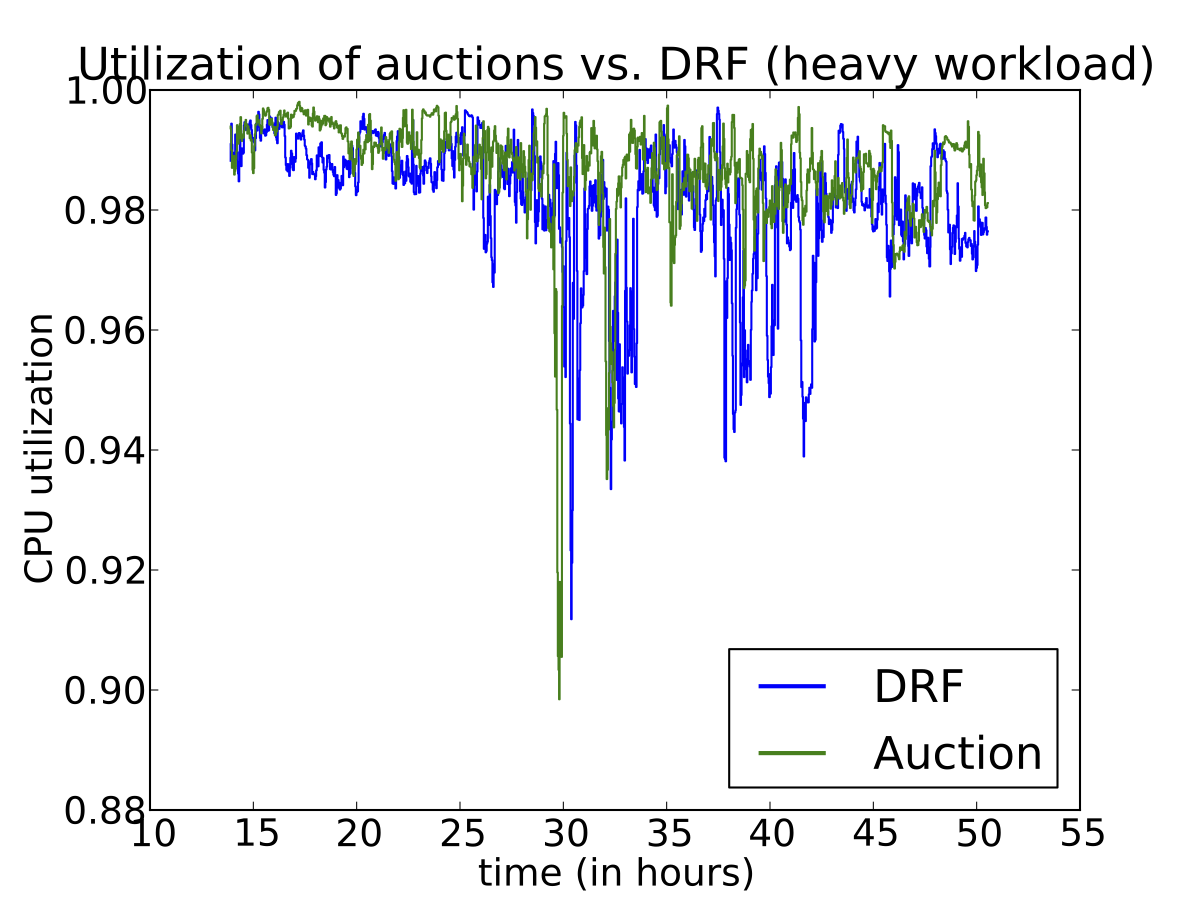
\includegraphics[width=0.5\textwidth]{images/util_high.png}
\caption{Utilization achieved by DRF and our policy on a simulated 25-node CPU-bound cluster.  DRF's average utilization is 98\% average utilization while ours is 99\%.}
\label{img:util_high}
\end{figure}

\begin{figure}

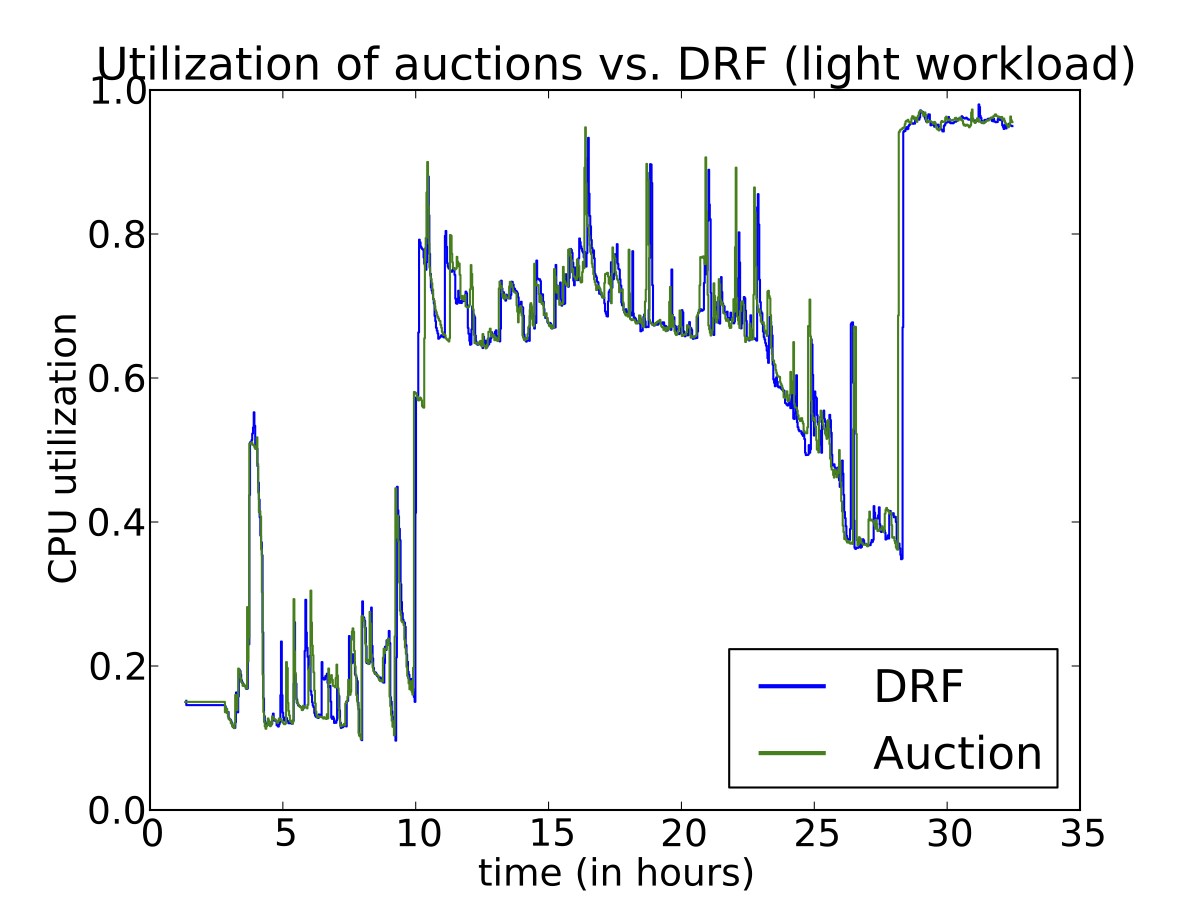
\includegraphics[width=0.5\textwidth]{images/util_low.png}
\caption{Behavior of DRF and our policy on a simulated 100-node cluster. Both policies have average utilization of 44\%.}
\label{img:util_low}
\end{figure}

\begin{figure}

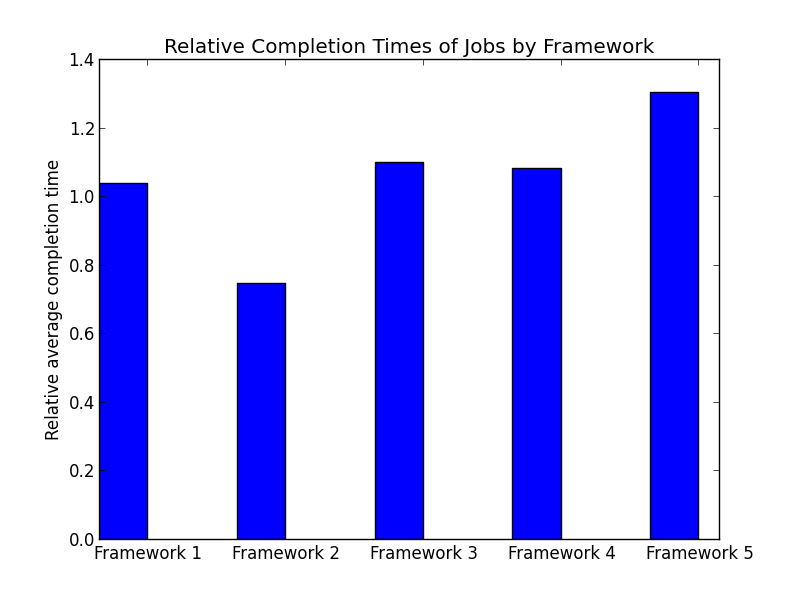
\includegraphics[width=0.5\textwidth]{images/relative_completion_times.png}
\caption{Relative average job completion times between DRF and auctions for all frameworks.}
\label{img:relative}
\end{figure}

Currently, Mesos jobs and tasks are not attached to economic indicators, since DRF does not rely on any economic-based resource scheduler. Even if a market-based mechanism was used, many cluster jobs and tasks may not be able or willing to provide accurate pricing data. In the absence of this information, our scheme provides a default bidding policy. This ``backwards-compatible'' mode must still perform comparable with DRF, especially given the current state of job requests.

To investigate this feature, we ran our simulator using both DRF and the market-based mechanism under the default bidding policy. We ran under two cluster environments, a 25-node cluster to simulate high resource contention, and a 100-node cluster to simulate a light workload. All nodes were homogeneous, with normalized CPU, RAM, and disk resources of 1. We ran using a statistical workload for five computing frameworks, each submitting 20 jobs in parallel. For each environment, we evaluated the resource utilization and job completion times of DRF and the market-based mechanism.

Figure \ref{img:util_high} shows the CPU utilizations of DRF and the market-based mechanism in the high contention environment.  The utilizations achieved by DRF and the default bidding policy are nearly identical. The average DRF utilization is approximately 98\%, while the market-based mechanism is approximately 99\%. Note the graph begins after 10 hours, when consistent maximum contention is reached. We elide the memory utilizations graph because it is not under high contention, as the Google traces indicate jobs are CPU bound, and looks similarly to Figure \ref{img:util_low}. However, it shows again the nearly identical performance between DRF and the market-based mechanism. Similarly, we do not show the disk utilization because very few jobs in the Google traces used local disk space (presumably instead relying on a Google-internal reliable file system).

Figure \ref{img:util_low} shows the CPU utilizations of DRF and the market-based mechanism in a low contention environment, when no resource is fully utilized. As we can see, DRF and the market-based mechanism perform nearly identical. Both policies have an average CPU utilization of 44\%. Again, we omit the memory and disk utilizations figures because they repeat the same story, but are less interesting due to the lower RAM and disk resource requirements of jobs.

Finally, Figure \ref{img:relative} displays the relative average job completion time between DRF and the market-based mechanism for the five frameworks. As we see, the ratio is roughly 1.0 for all frameworks, which indicates the market-based mechanism is roughly as fair as DRF, and that jobs complete at the same approximate rate.

All of these results are gathered when the market-based mechanism uses a default bidding policy because the job requests provide no economic information. This shows that the market-based mechanism is ``backwards-compatible" by providing comparable utilization and fairness performances to DRF when pricing information is not used. This result is not completely surprising though, because the default bidding policy behaves similarly to DRF. DRF awards resources to the framework with the least dominant share. Under our default bidding policy, frameworks bid a proportion of their current budget. The framework that has been awarded the least resources will have the highest budget (through less spending on resources), and will be able to bid the highest. Hence the low-resource framework will be awarded the next resource offer, similarly to DRF.

\subsection{Performance With Pricing\\}

When pricing information is provided, we show that the market-based mechanism can provide better performance than in DRF. As discussed in Section TODO, there are many situations in which prices can be used to better encapsulate a framework's preferences. As a case study, we investigate one particular scenario of inhomogeneous performing resources. 

In this case, we assume certain nodes have a special resource that significantly improves job performances, while the remaining nodes do not. In a realistic case, this special resource could be a GPU, which can significantly reduce CPU-bounded job completion times. While most jobs will see some performance benefits from running on a GPU, some jobs may be specifically crafted for optimal performance on a GPU, and hence will see the largest performance improvement if run on a GPU.

The current Mesos implementation does not recognize this special sort of inhomogeneous performing resource. However, if a framework is aware of the inhomogeneous performing resource, it can schedule tasks appropriately on slaves when offered, such that the tasks that benefit most from special resources will be scheduled on special resource slaves. For the simulations, we have implemented the framework scheduler in such a manner. For the market-based mechanism, we use a bidding policy proportional to the default bidding policy. However, when a task can benefit from a special slave by a speedup factor $s$, the default bid is multiplied by $\frac{1}{s}$, resulting in a bid that is inversely proportional to the speedup factor.

We simulate this scenario using a 64-node cluster, where 16 nodes have the special resource. Jobs from the statistical workload are uniformly randomly assigned one of two speedup factors, such that all tasks in a job experience the same speedup factor. The ``slow" speedup reduces task runtime by 10\%, while the ``fast" speedup reduces task runtime by 90\%. All tasks with a ``fast" speedup are marked as preferring a special resource slave, and a framework in DRF Mesos will schedule a ``fast" task on a special resource slave if possible. The workload was again generated for five frameworks, with up to 20 jobs running in parallel.

Figure \ref{img:inhomo} depicts the time progression of job completions, where a job is considered finished when all of its tasks are finished. As the figure depicts, the market-based mechanism is consistently ahead of DRF at all times, and finishes all jobs in about 20\% less time than DRF. Looking in detail, we find that DRF schedules only 30\% of ``fast" tasks on special resource slaves, while the market-based mechanism schedules 60\%. One might note that around the eighth hour, it appears DRF catches up to the market-based mechanism before falling behind again. This effect is caused by a long running job that the market-based mechanism schedules earlier than DRF. Its completion progresses the fraction of job completion minimally yet accounts for a long period of time. This allows DRF, which is still completing earlier short-lived tasks, to momentarily catch up in the fraction of job completion. When DRF schedules the same long-lived job at a latter point, it once again lags behind the market-based mechanism.

Hence, in the case of inhomogeneous performing resources, the market-based mechanism can allow frameworks to better express their preferences than DRF, resulting in better performance for the market-based mechanism. DRF only allows a framework to specifically target special resource slaves when the framework is offered, whereas the market-based mechanism allows frameworks who benefit most from a special resource slave to outbid others. By better scheduling jobs on machines that best complete them, we see the overall performance improvements of the market-based mechanism.


\begin{figure}
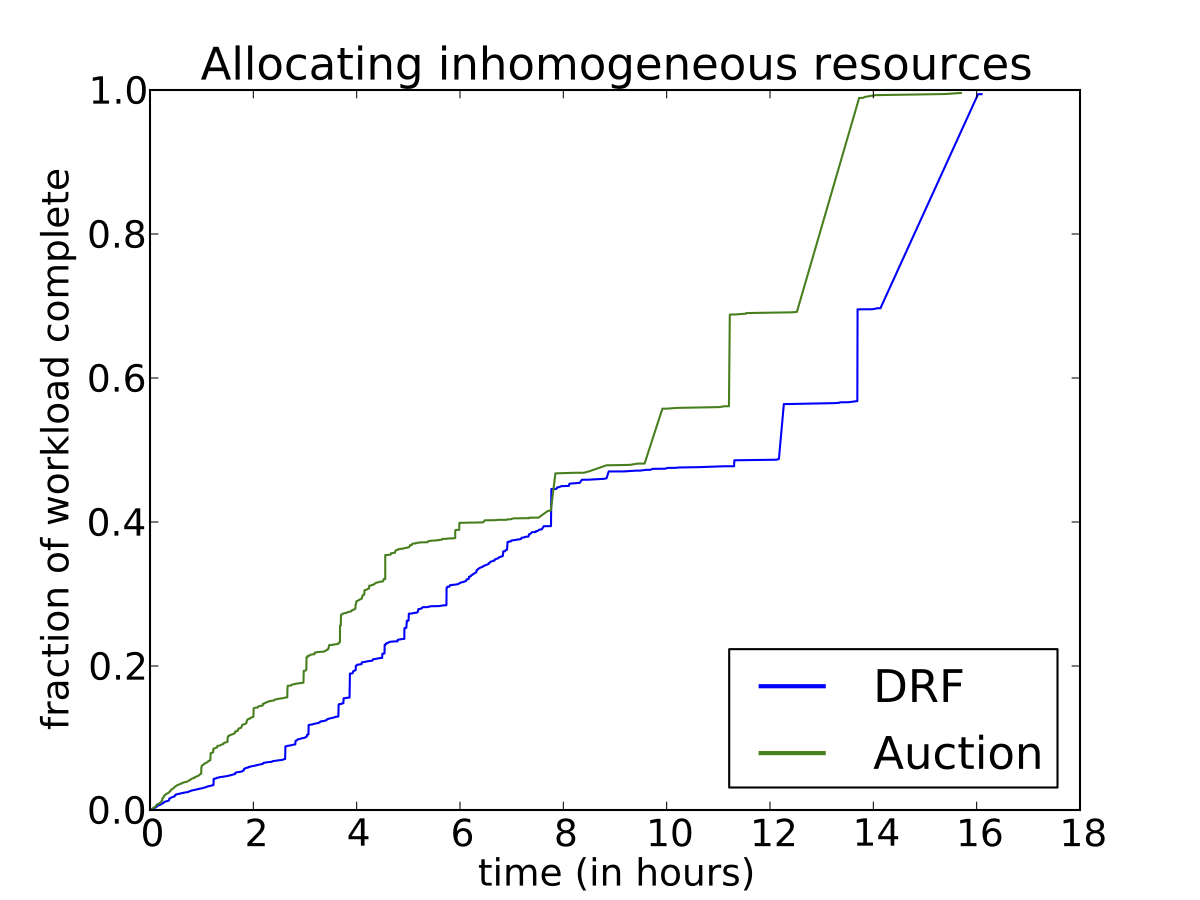
\includegraphics[width=0.5\textwidth]{images/inhomo_times.png}
\caption{The results of simulating Mesos on a cluster of 64 machines, of which 16 have access to a special resource. DRF schedules 30\% of tasks on the optimal machine when frameworks prioritize appropriately, while a simple market-based policy schedules 60\%.}
\label{img:inhomo}
\end{figure}


\section{Related Work}
\label{sec:related}

\subsection{Grid computing}
Job schedulers like TORQUE \cite{torque}, Condor \cite{condor}, and LSF
\cite{lsf} have long been used for solving the problem of resource allocation
within a high-performance-computing (HPC) or grid-computing environment.
For the most part, they do not use a two-level scheduling model like we do but
instead operate as a queue for predefined jobs which are run as resources become
available. Machines and job requirements also tend to show more homogeniety
within such environments (for example, the ratio between CPU, memory, and disk),
so sthe amount of optimization possible with pricing is lower.

\subsection{Cloud and datacenter computing}
Our work depends heavily on Mesos~\cite{mesos}, as we use its model of
resources, tasks, and frameworks as the basis for our own. We also use Mesos as
a baseline for purposes of comparison, as we have already extensively discussed.

Jockey~\cite{jockey} attempts to solve the specific problem of adjusting
resource allocation in the datacenter environment to ensure important jobs
finish within deadlines. They do not directly modify the scheduler for this but
instead adjust the priority of each job as needed within an existing system.
With our work, we attempt to create a general-purpose system which can solve not
only the problem of deadlines, but also allow expression of many different kinds
of demands and have them all interact nicely with each other without needing
specialized logic to keep track of each one explicitly.

\subsection{Resource allocation}
Dominant resource fairness~\cite{drf} is an allocation policy whereby the user with the smallest dominant share is next allocated resources. The user's dominant share in a multi-resource environment is the largest share the user possesses of any of the cluster's various resources.

\subsection{Economics/pricing in computer systems}
Lottery scheduling

\subsection{Economics/pricing for resource allocation}
Many previous researchers have proposed systems which use ideas from economics
to assign resources in computer systems.  Analogous to our datacenter
implementation, \cite{stoica94} uses prices, budgets, and auctions for
scheduling within a single machine. It ensures some level of fairness and
allows low-income but mostly-idle users to occasionally spend more money beyond
their income for urgent jobs by drawing upon their account balance. However,
resource demands are much more homogeneous in this environment than within a
datacenter, so the usefulness of prices as a vehicle for expressing prices are
more limited. Spawn \cite{spawn} uses auctions to rent time-slices of idle
workstations; rather than using prices as a priority-indicating mechanism
automatically set based on application requirements, this work places more
emphasis on using it for reimbursement where users manually allocate budgets to
jobs. Tycoon \cite{tycoon} also uses auctions to divide up the cluster's
resources among competing users, except the auctions are used for CPU scheduling
within each individual machine rather than for setting bounds on allowed
resource usage of each job, and has no provision for the presence of
multiple contentious resources.

More generally, fair division is the problem in economics of dividing a set of
resources equitably among a set of people. Our problem differs somewhat from
fair division in that we don't seek to allocate every bit of the cluster to the
set of users. We assume that a user might be happy to have received nothing if
their value of gaining resources was too low compared to the others, since the
user keeps some amont of money unspent as a a result.

One of the economic fair division solutions is CEEI~\cite{moulin2004fair}, or
competitive equilibrium from equal incomes. This mechanism emulates a market
where participants initially receive an equal amount of resources and trade some
of them until each has the desired amount of resources. CEEI's use of a market
differs significantly from ours in that we do not use it only as a vehicle for
achieving a fair allocation, but also for frameworks to express their
preferences in a fine-grianed way using prices and willingness to pay.

\section{Future Work}
\label{sec:future}

In our evaluation, we showed through simulation the benefits of our protocol in the specific case of inhomogenous performing resources. However, there are a number of other user constraints that should theoretically be better expressed using prices than existing methods. Future work would be to experimentally evaluate such cases. A few such user constraints include deadlines and varying latency sensitivities, differential service guarantees, deadweight losses of evictions, costs of fragmenting jobs, various execution types (e.g. speculative vs essential execution), and co-location of data or other important resources.

\section{Conclusion}
\label{sec:conclusion}

This paper presented an initial investigation into the possibility of leveraging prices and a market-based mechanism for resource scheduling. We describe a protocol for use in the Mesos cluster scheduler with beneficial theoretical properties. Simulation evaluation shows that our market-based mechanism can perform reasonably in a backwards-compatible mode, where no economic information is provided. When economic data exists, our approach can provide substantial performance benefits.

\section{Acknowledgement}

We thank Professors Anthony Joseph and John Kubiatowicz for guidance and numerous suggestions throughout the course of this project. Also, we thank Charles Reiss for providing helpful tips on how best to use the Google cluster traces. Finally, we thank Ali Ghodsi for providing meaningful discussion into the theory behind our market-based mechanism.

%
% The following two commands are all you need in the
% initial runs of your .tex file to
% produce the bibliography for the citations in your paper.
\bibliographystyle{abbrv}
\bibliography{paper}  % sigproc.bib is the name of the Bibliography in this case
% You must have a proper ".bib" file
%  and remember to run:
% latex bibtex latex latex
% to resolve all references
%
% ACM needs 'a single self-contained file'!
%
%APPENDICES are optional
%\balancecolumns
%\appendix
%Appendix A
%\section{Headings in Appendices}
%The rules about hierarchical headings discussed above for
%the body of the article are different in the appendices.
%In the \textbf{appendix} environment, the command
%\textbf{section} is used to
%indicate the start of each Appendix, with alphabetic order
%designation (i.e. the first is A, the second B, etc.) and
%a title (if you include one).  So, if you need
%hierarchical structure
%\textit{within} an Appendix, start with \textbf{subsection} as the
%highest level. Here is an outline of the body of this
%document in Appendix-appropriate form:
%\subsection{Introduction}
%\subsection{The Body of the Paper}
%\subsubsection{Type Changes and  Special Characters}
%\subsubsection{Math Equations}
%\paragraph{Inline (In-text) Equations}
%\paragraph{Display Equations}
%\subsubsection{Citations}
%\subsubsection{Tables}
%\subsubsection{Figures}
%\subsubsection{Theorem-like Constructs}
%\subsubsection*{A Caveat for the \TeX\ Expert}
%\subsection{Conclusions}
%\subsection{Acknowledgments}
%\subsection{Additional Authors}
%This section is inserted by \LaTeX; you do not insert it.
%You just add the names and information in the
%\texttt{{\char'134}additionalauthors} command at the start
%of the document.
%\subsection{References}
%Generated by bibtex from your ~.bib file.  Run latex,
%then bibtex, then latex twice (to resolve references)
%to create the ~.bbl file.  Insert that ~.bbl file into
%the .tex source file and comment out
%the command \texttt{{\char'134}thebibliography}.
%% This next section command marks the start of
%% Appendix B, and does not continue the present hierarchy
%\section{More Help for the Hardy}
%The acm\_proc\_article-sp document class file itself is chock-full of succinct
%and helpful comments.  If you consider yourself a moderately
%experienced to expert user of \LaTeX, you may find reading
%it useful but please remember not to change it.
\balancecolumns
% That's all folks!
\end{document}
